% Report for IoT Lab 2 -- Activity 2
\documentclass[11pt,a4paper]{article}
\usepackage[utf8]{inputenc}
\usepackage[T1]{fontenc}
\usepackage[english]{babel}
\usepackage[margin=2cm]{geometry}
\usepackage{graphicx}
\usepackage{float}
\usepackage{pgfplots}
\usepackage{listings}
\usepackage{parskip}
\usepackage{booktabs}
\usepackage{caption}
\usepackage{subcaption}
\usepackage{enumitem}
\captionsetup{font=small}
\captionsetup[subfigure]{font=small}
\setlist{itemsep=1pt, topsep=2pt}
\usepackage{hyperref}
\usepackage{textcomp}
\usetikzlibrary{positioning,arrows.meta,calc,fit}
\pgfplotsset{compat=1.18}
\lstset{breaklines=true,basicstyle=\ttfamily\footnotesize,frame=single,columns=fullflexible}
\hypersetup{colorlinks=true,linkcolor=blue,urlcolor=blue}
\emergencystretch=3em

% Common style of the plots.
\pgfplotsset{lab/.style={
  width=\textwidth, height=4.6cm,
  grid=major, grid style={gray!25},
  tick label style={font=\scriptsize}, label style={font=\scriptsize},
  legend style={font=\scriptsize}, title style={font=\small},
}}

\title{\textbf{Activity 2: LoRa-based communication with MQTT integration}}
\author{Omar Antonio Cornejo Vargas}
\date{13 October 2026}

\begin{document}
\maketitle

\section{Introduction}

Activity~1 built a telemetry chain in which one ESP32 read a DHT11 sensor and published the
readings directly to an MQTT broker over Wi-Fi. Activity~2 adds a LoRa radio link to that
chain: a first ESP32 (the \emph{sensor node}) reads the DHT11 and sends the reading over LoRa
at 868~MHz, and a second ESP32 (the \emph{gateway}) receives it and publishes it to the MQTT
broker. The goals are to implement this link, to study how bandwidth, spreading factor and
transmission power affect speed, range, energy and signal quality, and to measure the packet
loss over distance.


%=====================================================================
\section{System overview}
\label{sec:arch}

Figure~\ref{fig:arch} shows the architecture. Only the two boards and the LoRa link are new:
the sensor node no longer needs Wi-Fi, and the gateway is the only board on the network.

\begin{figure}[H]
\centering
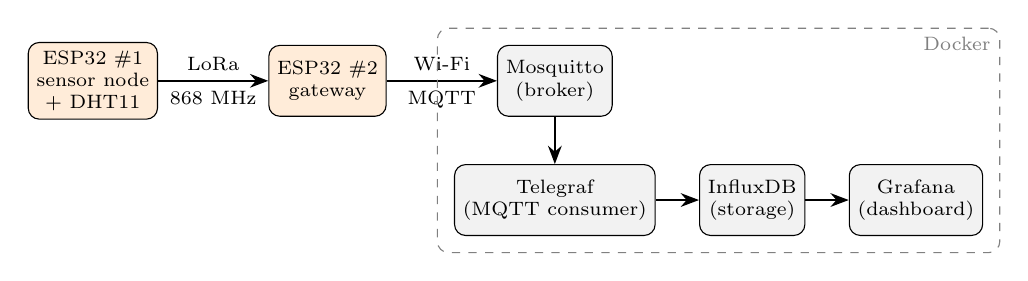
\begin{tikzpicture}[
  node distance=0.55cm and 0.55cm,
  box/.style={draw, rounded corners, align=center, font=\scriptsize, minimum height=0.9cm, inner sep=3pt},
  new/.style={box, fill=orange!15},
  old/.style={box, fill=gray!10},
  arr/.style={-{Stealth}, thick},
]
\node[new] (sensor) {ESP32 \#1\\sensor node\\+ DHT11};
\node[new, right=1.4cm of sensor] (gw) {ESP32 \#2\\gateway};
\node[old, right=1.4cm of gw] (mosq) {Mosquitto\\(broker)};
\node[old, below=0.6cm of mosq] (tele) {Telegraf\\(MQTT consumer)};
\node[old, right=of tele] (influx) {InfluxDB\\(storage)};
\node[old, right=of influx] (graf) {Grafana\\(dashboard)};
\draw[arr] (sensor) -- node[above, font=\scriptsize]{LoRa} node[below, font=\scriptsize]{868 MHz} (gw);
\draw[arr] (gw) -- node[above, font=\scriptsize]{Wi-Fi} node[below, font=\scriptsize]{MQTT} (mosq);
\draw[arr] (mosq) -- (tele);
\draw[arr] (tele) -- (influx);
\draw[arr] (influx) -- (graf);
\node[draw, dashed, gray, rounded corners, inner sep=6pt, fit=(mosq)(tele)(influx)(graf)] (docker) {};
\node[font=\scriptsize, gray, anchor=north east] at (docker.north east) {Docker};
\end{tikzpicture}
\caption{Architecture. Orange: new in this activity. Grey: reused from Activity~1.}
\label{fig:arch}
\end{figure}

A reading changes as follows on its way through the system: the sensor node sends the first
JSON over LoRa, the gateway adds the link quality and publishes the second one, and InfluxDB
stores the third line in the measurement \texttt{lora\_weather}:

\begin{lstlisting}
LoRa:      {"seq":52,"temperature":26.20,"humidity":72.00}
MQTT:      {"seq":52,"temperature":26.20,"humidity":72.00,"rssi":-33,"snr":9.5,"lost":0}
InfluxDB:  lora_weather,host=<container> seq=52,temperature=26.2,humidity=72,rssi=-33,snr=9.5,lost=0 <ts>
\end{lstlisting}

The new fields are \texttt{seq} (sequence number added by the sender), \texttt{rssi} and
\texttt{snr} (signal strength and signal-to-noise ratio measured by the gateway), and
\texttt{lost} (lost packets counted by the gateway, Section~\ref{sec:gw}).

%=====================================================================
\section{Reused from Activity 1}
\label{sec:reuse}

The server side and the sensor reading were reused from Activity~1 with small changes.

\begin{table}[H]
\centering
\small
\begin{tabular}{p{3.3cm}p{13.3cm}}
\toprule
\textbf{Component} & \textbf{Change in Activity 2} \\
\midrule
DHT11 reading & Same code (pin~33, \texttt{isnan()} validation), now only on the sensor node. \\
Wi-Fi + MQTT client & Same \texttt{PubSubClient} logic, moved to the gateway. New topic \texttt{sensor/esp01\_lora}. \\
JSON payload & Same single-object format, with the new fields \texttt{seq}, \texttt{rssi}, \texttt{snr}, \texttt{lost}. \\
\texttt{docker-compose.yml} & Same four services. New container names, host ports (1884, 8087, 3001) and database \texttt{lora\_db}, so both labs can run at the same time. \\
Telegraf & Same JSON consumer, only \texttt{name\_override = "lora\_weather"} changed. New fields are stored automatically. \\
Grafana & Same provisioning. New dashboard \emph{LoRa Weather Station} (Figure~\ref{fig:grafana-overview}): temperature and humidity, plus RSSI, SNR and QoS panels (received/lost packets, loss rate, sequence number and an OK/LOST status per packet). \\
\bottomrule
\end{tabular}
\caption{Parts reused from Activity~1 and the changes made to them.}
\label{tab:reuse}
\end{table}

\begin{figure}[H]
\centering
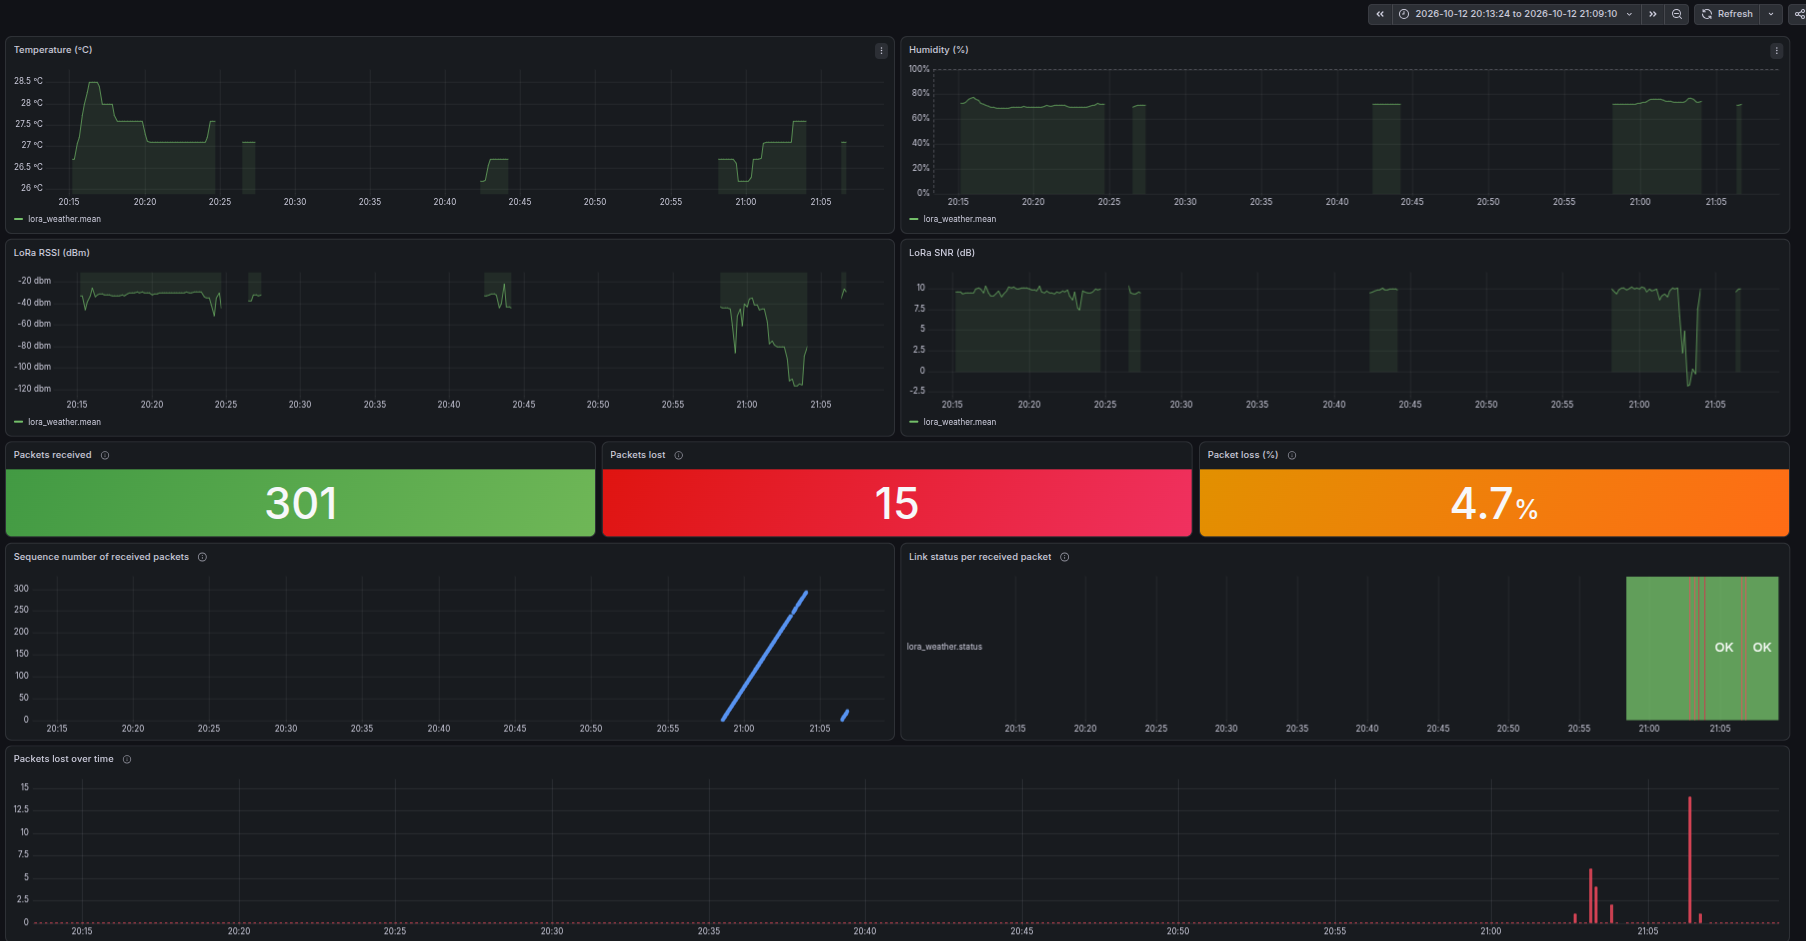
\includegraphics[width=\textwidth]{img/grafana_overview.png}
\caption{Grafana dashboard \emph{LoRa Weather Station}.}
\label{fig:grafana-overview}
\end{figure}

%=====================================================================
\section{Implementation of the LoRa link}
\label{sec:lora}

\subsection{Hardware and Radio configuration}

Both boards are \textbf{Heltec WiFi LoRa 32 V2}, which have the LoRa radio already built in.
Only the sensor node has the DHT11 connected, to read the temperature and the humidity. Both
boards are plugged into the PC by USB, but only to get power. The data only reaches the PC
through the gateway, which is the only board connected via Wi-Fi to the MQTT broker running on
the PC.

LoRa has no negotiation: the receiver only decodes a packet if it uses \textbf{exactly the
same parameters} as the transmitter. They are declared as constants at the top of both
sketches, so every change of BW or SF requires re-uploading both boards (the TX power only
affects the sender).

\begin{table}[H]
\centering
\small
\begin{tabular}{ll}
\toprule
Parameter & Value\\
\midrule
Frequency & 868.0 MHz\\
Bandwidth (BW) & 125 / 250 / 500 kHz\\
Spreading factor (SF) & 7 / 9\\
Coding rate (CR) & 4/5\\
Preamble & 8 symbols\\
Sync word & \texttt{0x12}\\
TX power & 7 / 10 / 14 dBm\\
\bottomrule
\end{tabular}
\caption{LoRa parameters.}
\label{tab:params}
\end{table}

\subsection{Sensor node firmware (ESP32 \#1)}

\texttt{sketch\_lora\_sender.ino}:
\begin{enumerate}
  \item Starts the DHT11 and the radio with the parameters of Table~\ref{tab:params}. If
        \texttt{radio.begin()} fails it stops and prints the error code.
  \item Every second, reads and validates the DHT11 (same code as Activity~1).
  \item Builds the JSON with an increasing sequence number \texttt{seq}, which lets the
        gateway detect lost packets.
  \item Sends it with \texttt{radio.transmit()}, which blocks until the transmission ends.
  \item Prints the time on air (\texttt{getTimeOnAir()}) and the estimated energy of the
        packet (Section~\ref{sec:power}).
\end{enumerate}

\subsection{Gateway firmware (ESP32 \#2)}
\label{sec:gw}

\texttt{sketch\_lora\_receiver.ino}:
\begin{enumerate}
  \item Starts the SPI bus and the radio with the same parameters as the sender.
  \item Registers an interrupt routine with \texttt{setPacketReceivedAction()} that only sets
        a flag when a packet arrives, and puts the radio in continuous reception.
  \item Connects to Wi-Fi and MQTT with the code reused from Activity~1.
  \item When the flag is set, reads the packet with \texttt{readData()}. A packet with a wrong
        CRC is counted as \emph{invalid} and discarded. Otherwise it reads the RSSI and SNR,
        checks the sequence number (a jump bigger than one adds the missing packets to
        \texttt{lost}), appends \texttt{rssi}, \texttt{snr} and \texttt{lost} to the JSON and
        publishes it. Then it goes back to reception mode.
\end{enumerate}

\textbf{Problem found:} at first the loss was estimated by comparing the packet counters of
both boards, but they never matched because the boards were restarted at different moments.
\textbf{Solution:} the sequence number inside the packet, so the gateway calculates the loss
on its own.

%=====================================================================
\section{Experiments on LoRa parameters}
\label{sec:exp}

\textbf{Common method.} The RSSI and SNR of every packet were taken from the Serial monitor
of the gateway and saved in \texttt{data/lora\_samples.csv}. Three
reference positions were used inside the room, \emph{close} (a few centimetres),
\emph{medium} (normal desk distance) and \emph{far} (the maximum distance the setup allowed, away from the PC). As the
boards were placed by hand, the same position can vary a few dB between tests. The RSSI is
the received power, the SNR compares the signal with the noise, and
LoRa can decode packets with a negative SNR.

%---------------------------------------------------------------------
\subsection{Experiment 1: bandwidth and data rate}
\label{sec:bw}

In this experiment only the bandwidth (\texttt{LORA\_BANDWIDTH}) and the spreading factor
(\texttt{LORA\_SPREADING\_FACTOR}) were changed, at 14~dBm, and three combinations were tested
in the three positions: \textbf{BW~125~kHz with SF7}, \textbf{BW~250~kHz with SF9} and
\textbf{BW~500~kHz with SF9}.

\begin{figure}[H]
\centering
\begin{subfigure}[b]{0.48\textwidth}
\centering
\begin{tikzpicture}
\begin{axis}[lab,
    ybar, bar width=7pt,
    symbolic x coords={BW125-SF7,BW250-SF9,BW500-SF9}, xtick=data,
    ylabel={Mean RSSI (dBm)}, ymin=-60, ymax=0,
    enlarge x limits=0.25,
    legend style={at={(0.5,1.03)}, anchor=south, font=\scriptsize}, legend columns=3,
]
\addplot[fill=blue!50]  table [col sep=comma, x=config, y=rssi_close]  {data/bw_sf_summary.csv};
\addplot[fill=blue!25]  table [col sep=comma, x=config, y=rssi_medium] {data/bw_sf_summary.csv};
\addplot[fill=gray!30]  table [col sep=comma, x=config, y=rssi_far]    {data/bw_sf_summary.csv};
\legend{close, medium, far}
\end{axis}
\end{tikzpicture}
\caption{Mean RSSI per position.}
\label{fig:bw-rssi}
\end{subfigure}
\hfill
\begin{subfigure}[b]{0.48\textwidth}
\centering
\begin{tikzpicture}
\begin{axis}[lab,
    ybar, bar width=7pt,
    symbolic x coords={BW125-SF7,BW250-SF9,BW500-SF9}, xtick=data,
    ylabel={Mean SNR (dB)}, ymin=5, ymax=15,
    enlarge x limits=0.25,
    legend style={at={(0.5,1.03)}, anchor=south, font=\scriptsize}, legend columns=3,
]
\addplot[fill=blue!50]  table [col sep=comma, x=config, y=snr_close]  {data/bw_sf_summary.csv};
\addplot[fill=blue!25]  table [col sep=comma, x=config, y=snr_medium] {data/bw_sf_summary.csv};
\addplot[fill=gray!30]  table [col sep=comma, x=config, y=snr_far]    {data/bw_sf_summary.csv};
\legend{close, medium, far}
\end{axis}
\end{tikzpicture}
\caption{Mean SNR per position.}
\label{fig:bw-snr}
\end{subfigure}
\caption{Experiment 1: received signal of each BW/SF configuration (\texttt{data/bw\_sf\_summary.csv}).}
\label{fig:bw}
\end{figure}

\textbf{Results and discussion.} In theory, a wider bandwidth makes the transmission faster
but lets more noise into the channel, so the SNR is lower. A higher SF makes each packet
slower but more robust, and a narrower channel with a higher SF gives the best sensitivity and
therefore the longest range. During the experiment it was not possible to record every value, but what was observed and the values
that could be captured follow this behaviour:
\begin{itemize}
  \item \textbf{Fastest configuration: BW~500~kHz with SF9.} With the widest channel the
        packets were sent and received faster than with the other two configurations, but
        they arrived with the most noise: it gave the lowest SNR, about 7.6~dB
        (Figure~\ref{fig:bw-snr}).
  \item \textbf{Best signal: BW~250~kHz with SF9.} It was the slowest configuration, but it
        received the cleanest signal, with the highest SNR (about 13~dB) in all three
        positions. With a narrower channel and SF9, it is also the configuration with the
        longest range in theory.
  \item \textbf{BW~125~kHz with SF7} was in the middle, with an SNR of about 9.7~dB.
\end{itemize}
In short, increasing the bandwidth gives speed, while increasing the SF gives a more robust
signal and therefore more range. For a weather station that only sends a few bytes, range
usually matters more than speed.


%---------------------------------------------------------------------
\subsection{Experiment 2: transmission power}
\label{sec:power}

With BW~125~kHz and SF7 fixed, the sender power was set to 7, 10 and 14~dBm and the RSSI/SNR
were recorded in the three positions. No multimeter was available, so the energy per packet
is estimated as $E = V \cdot I_{tx} \cdot t_{air}$, with $V = 3.3$~V and $t_{air} = 83$~ms
calculated exactly by RadioLib. $I_{tx}$ is the estimated
part: the SX1276 datasheet gives 87~mA at 17~dBm and 120~mA at 20~dBm, and
the values for 7, 10 and 14~dBm (45, 55, 80~mA) were estimated from them. The absolute energy
and the comparison between powers are therefore only valid according to the estimated currents.

\begin{figure}[H]
\centering
\begin{subfigure}[b]{0.48\textwidth}
\centering
\begin{tikzpicture}
\begin{axis}[lab,
    ybar, bar width=16pt,
    symbolic x coords={7,10,14}, xtick=data,
    xlabel={TX power (dBm)}, ylabel={Energy per packet (mJ)}, ymin=0, ymax=26,
    nodes near coords, nodes near coords style={font=\scriptsize},
    enlarge x limits=0.3,
]
\addplot[fill=teal!50, draw=teal!70!black] table [col sep=comma, x=tx_power_dbm, y=energy_mj] {data/tx_power_summary.csv};
\end{axis}
\end{tikzpicture}
\caption{Energy per packet ($t_{air} = 83$ ms).}
\label{fig:pw-energy}
\end{subfigure}
\hfill
\begin{subfigure}[b]{0.48\textwidth}
\centering
\begin{tikzpicture}
\begin{axis}[lab,
    xlabel={TX power (dBm)}, ylabel={Mean RSSI (dBm)},
    xmin=6, xmax=15, xtick={7,10,14}, ymin=-60, ymax=-10,
    legend style={at={(0.5,1.03)}, anchor=south, font=\scriptsize}, legend columns=4,
]
\addplot+[thick, mark=*, blue!70!black]      table [col sep=comma, x=tx_power_dbm, y=rssi_close]  {data/tx_power_summary.csv};
\addplot+[thick, mark=square*, blue!40]      table [col sep=comma, x=tx_power_dbm, y=rssi_medium] {data/tx_power_summary.csv};
\addplot+[thick, mark=triangle*, gray]       table [col sep=comma, x=tx_power_dbm, y=rssi_far]    {data/tx_power_summary.csv};
\addplot[dashed, red, domain=7:14] {-35.2 + (x-7)};
\legend{close, medium, far, ideal +1 dB/dB}
\end{axis}
\end{tikzpicture}
\caption{Mean RSSI against TX power.}
\label{fig:pw-rssi}
\end{subfigure}
\caption{Experiment 2: energy and received signal for each power (\texttt{data/tx\_power\_summary.csv}).}
\label{fig:pw}
\end{figure}

\textbf{Results and discussion.}
\begin{itemize}
  \item \textbf{Energy.} According to the estimated currents, from 7 to 14~dBm the energy per
        packet grows 78\% (12.3 to 21.9~mJ), while the radiated power is multiplied by 5.
  \item \textbf{Signal strength.} At \emph{medium} and \emph{far} the RSSI improves by 3.7
        and 5.9~dB, close to the ideal 7~dB (Figure~\ref{fig:pw-rssi}). At \emph{close} there
        is no clear trend: with a few centimetres between antennas the receiver is saturated
        and the RSSI is not reliable. The SNR stays at 9.4--10~dB in all cases.
  \item \textbf{Usefulness.} With a margin of about 70~dB already at 7~dBm, the extra power
        only spent energy. More power only makes sense near the sensitivity limit.
\end{itemize}

\begin{figure}[H]
\centering
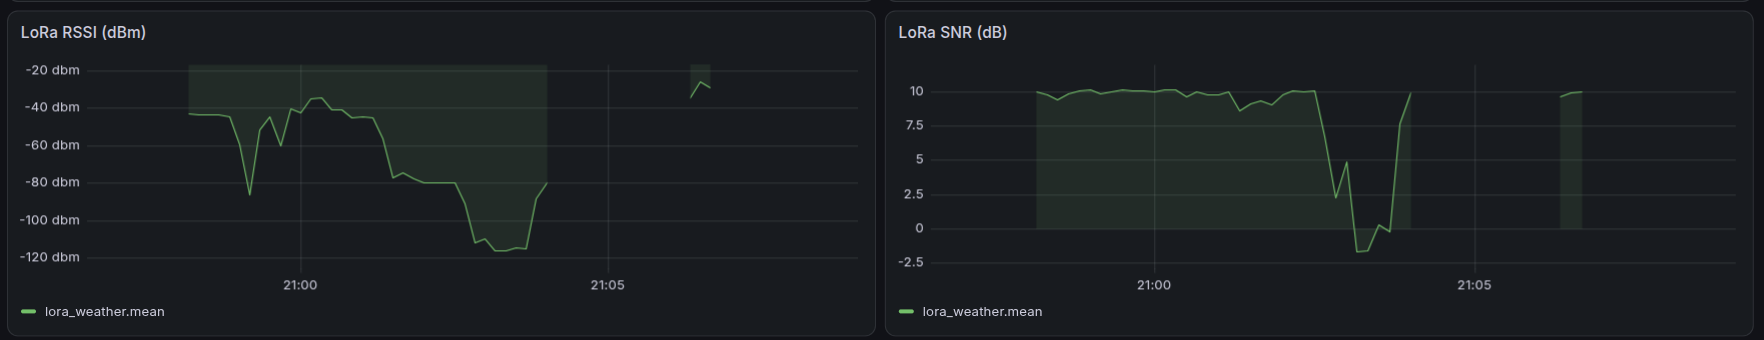
\includegraphics[width=\textwidth]{img/grafana_rssi_snr.png}
\caption{Grafana RSSI and SNR panels over the whole session, including the QoS test of
experiment~3.
Each step in the curves is a change of configuration, TX power, position or foil. The values of
each test are taken from the Serial logs of the gateway.}
\label{fig:grafana-exp12}
\end{figure}

%---------------------------------------------------------------------
\subsection{Experiment 3: quality of service (packet loss over distance)}
\label{sec:qos}

With BW~125~kHz, SF7 and 10~dBm, the loss was measured with the sequence number: every jump in
\texttt{seq} is a packet that never reached the gateway. At the \emph{far} position of the
previous experiments the link still had a large margin and lost no packets, and the setup did
not allow a longer distance. To bring the link to its limit, the boards were kept at the
\emph{far} position and wrapped in aluminium foil, which attenuates the signal as a much longer
distance would. Three scenarios were compared: \emph{close} (a few centimetres, no foil),
\emph{far + foil (partial)} and \emph{far + foil
(full)}. For each one, a window of
consecutive packets was taken from the gateway log (\texttt{data/qos\_packets.csv}).

\begin{table}[H]
\centering
\small
\begin{tabular}{lcccccc}
\toprule
Scenario & Seq. window & Sent & Received & Lost & Loss (\%) & RSSI min / SNR min \\
\midrule
Close               & 10--18   & 9  & 9  & 0 & 0.0  & $-28$~dBm / 8.8~dB \\
Far + foil (partial) & 230--240 & 11 & 11 & 0 & 0.0  & $-118$~dBm / $-2.7$~dB \\
Far + foil (full)    & 280--289 & 10 & 8  & 2 & 20.0 & $-122$~dBm / $-5.5$~dB \\
\bottomrule
\end{tabular}
\caption{Packet loss of each scenario (\texttt{data/qos\_summary.csv}).}
\label{tab:qos}
\end{table}

\begin{figure}[H]
\centering
\begin{subfigure}[b]{0.48\textwidth}
\centering
\begin{tikzpicture}
\begin{axis}[lab,
    xlabel={Sequence number}, ylabel={RSSI (dBm)},
    xmin=229.5, xmax=240.5, ymin=-130, ymax=-70,
    restrict x to domain=230:240,
    legend pos=north west,
]
\addplot+[thick, mark=*, blue!70!black] table [col sep=comma, x=seq, y=rssi_dbm] {data/qos_packets.csv};
\addplot[dashed, red, thick, domain=229.5:240.5] {-124.5};
\legend{received, sensitivity SF7}
\end{axis}
\end{tikzpicture}
\caption{Far + foil (partial): no losses.}
\label{fig:qos-far}
\end{subfigure}
\hfill
\begin{subfigure}[b]{0.48\textwidth}
\centering
\begin{tikzpicture}
\begin{axis}[lab,
    xlabel={Sequence number}, ylabel={RSSI (dBm)},
    xmin=279.5, xmax=289.5, ymin=-130, ymax=-70,
    restrict x to domain=280:289,
    legend pos=north west,
]
\addplot+[thick, mark=*, blue!70!black] table [col sep=comma, x=seq, y=rssi_dbm] {data/qos_packets.csv};
\addplot[only marks, mark=x, mark size=4pt, red, very thick] table [col sep=comma, x=seq, y=marker] {data/qos_lost.csv};
\addplot[dashed, red, thick, domain=279.5:289.5] {-124.5};
\legend{received, lost, sensitivity SF7}
\end{axis}
\end{tikzpicture}
\caption{Far + foil (full): packets 283 and 285 lost.}
\label{fig:qos-shield}
\end{subfigure}
\caption{Experiment 3: RSSI of each received packet. Dashed line: theoretical sensitivity of
SF7 at 125~kHz ($-124.5$~dBm).}
\label{fig:qos}
\end{figure}

\textbf{Results and discussion.}
\begin{itemize}
  \item \textbf{Close:} no losses, RSSI around $-25$~dBm, 100~dB above the sensitivity.
  \item \textbf{Far + foil (partial):} the RSSI falls to between $-105$ and $-118$~dBm and the SNR becomes negative
        ($-2.7$~dB), but no packet is lost (Figure~\ref{fig:qos-far}). This is the main
        advantage of LoRa: it decodes packets below the noise level.
  \item \textbf{Far + foil (full):} the RSSI reaches $-122$~dBm and the SNR $-5.5$~dB, only
        2.5~dB and 2~dB above the limits (SF7 can decode down to $-7.5$~dB of SNR). Packets 283 and 285 were lost
        (Figure~\ref{fig:qos-shield}). For each one the gateway printed \texttt{code -7} (CRC
        mismatch), so the radio detected the packet but its bits were corrupted. When the
        foil was removed (packets 286--289) the RSSI went back to about $-80$~dBm and the
        losses stopped.
  \item \textbf{Behaviour.} The loss does not grow slowly with distance: the link works
        perfectly until the signal approaches the sensitivity, and then it fails suddenly.
\end{itemize}

\begin{figure}[H]
\centering
\begin{subfigure}[b]{\textwidth}
\centering
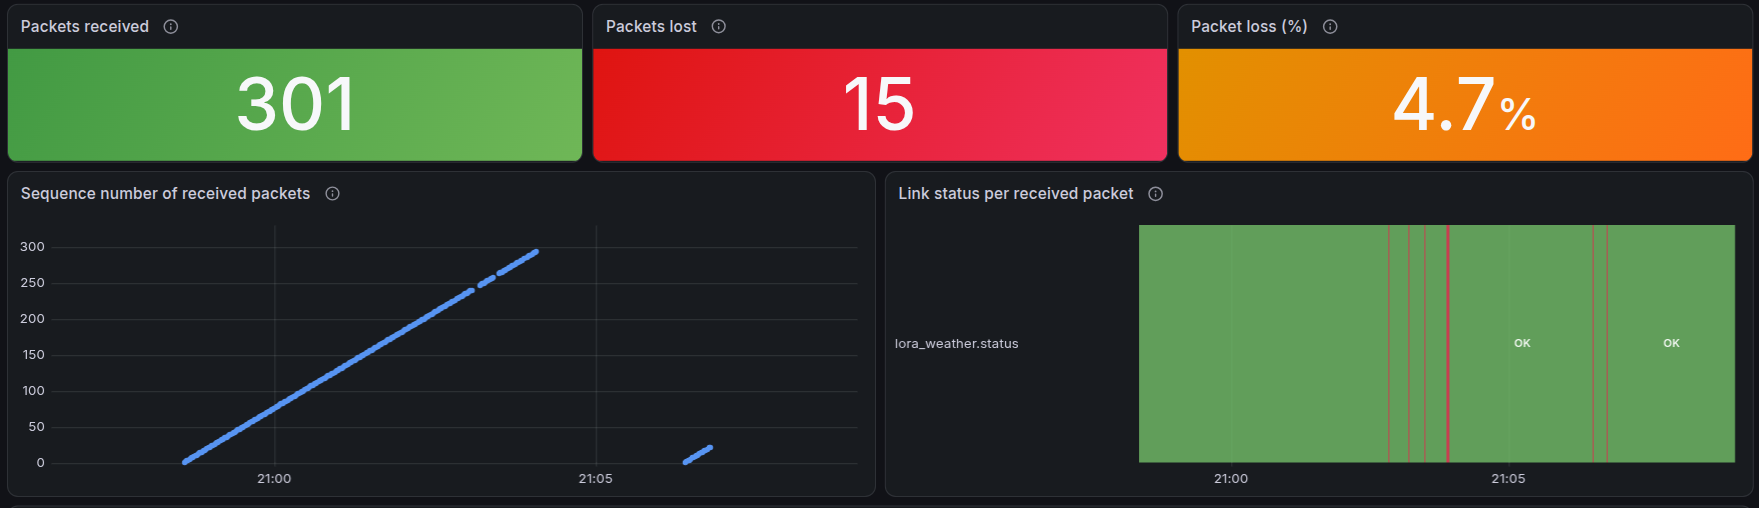
\includegraphics[width=0.9\linewidth]{img/grafana_qos_status.png}
\caption{Loss counters and link status per packet.}
\label{fig:grafana-qos-status}
\end{subfigure}

\vspace{0.3cm}
\begin{subfigure}[b]{\textwidth}
\centering
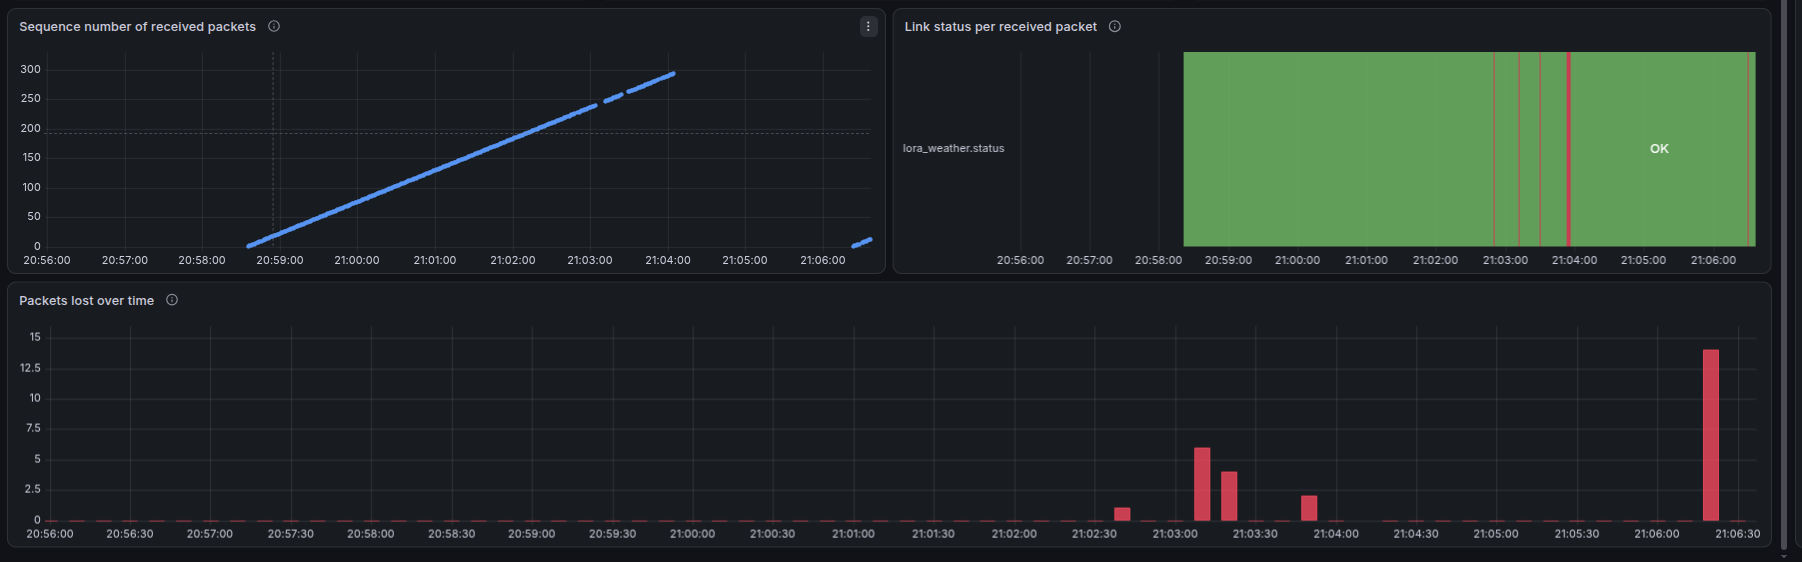
\includegraphics[width=0.9\linewidth]{img/grafana_qos_seq.png}
\caption{Sequence number and packets lost over time.}
\label{fig:grafana-qos-seq}
\end{subfigure}
\caption{Grafana QoS panels over the whole session. The counters are accumulated over the entire session, including the tests and the restarts of the
sender. The red marks in the link status and the bars of lost
packets show when the losses happened.}
\label{fig:grafana-qos}
\end{figure}

%=====================================================================
\section{Answers to the guiding questions}
\label{sec:questions}

\textbf{How does LoRa compare to Wi-Fi and Bluetooth in terms of range and power
consumption?}
LoRa has a much longer range. Wi-Fi usually reaches 50--100~m indoors and Bluetooth Low
Energy 10--50~m, while LoRa can cover several kilometres outdoors because it decodes signals
below the noise level. In our test the link still worked at $-118$~dBm, where Wi-Fi would
have disconnected long before. The price is the data rate: a few kbps, against tens of Mbps
for Wi-Fi. Regarding power, LoRa only consumes during short
bursts and can sleep the rest of the time, while Wi-Fi on the
ESP32 has to stay connected to the access point and keep listening, which consumes much more
power even when no data is sent.
BLE uses even less power, but only over short distances.

\textbf{What are the trade-offs of using lower data rates in LoRa transmission?}
A lower data rate makes the receiver more sensitive, so the
range and the robustness against noise increase. The drawback is that each packet stays
longer in the air, so it is slower and the radio spends more energy on it. A longer time on air also means fewer packets,
more collisions with other nodes and more latency. It is the right choice for small,
infrequent messages over long distances, but not for sending a lot of data.

\textbf{How does increasing transmission power affect battery life and interference?}
More power means more current, so the battery lasts less: in experiment~2, going from 7 to
14~dBm increased the estimated energy per packet by 78\%, while the RSSI only improved by 4--6~dB, and
with our 70~dB margin that energy was wasted. More power also increases interference: the
signal reaches further, so it can collide with other LoRa nodes on the same channel.

%=====================================================================
\section{Conclusions}
\label{sec:conclusions}

The LoRa link works end to end: the sensor node sends the DHT11 readings over LoRa, and the
gateway adds the link quality and a loss counter and publishes them to the Docker pipeline of
Activity~1. The experiments show the three trade-offs of
LoRa: bandwidth and spreading factor trade speed for signal quality,
transmission power trades energy for signal strength, and the quality of service depends on the margin over the sensitivity.

The code and the data are available at \url{https://github.com/omar-cornejo/EPSEM/tree/main/Iot/Lab2}.

\end{document}
